% LUMC presentation template by J. F. J. Laros.
% Last alteration on 15-10-2009.
%
% The packages texlive-latex-recommended, texlive-latex-base and
%   texlive-latex-extra should be installed.
%

% Alter these four lines for a new presentation.
\providecommand{\me}{Jeroen F. J. Laros}
\providecommand{\myFooter}{5th GA Meeting, Aveiro 11-12 January 2010}
\providecommand{\myTitle}{Web services for LOVD and Mutalyzer}

% Now go to %%% BEGIN PRESENTATION %%%

\documentclass[a4, portrait]{seminar}

\usepackage{semcolor} % For coloured text.
\usepackage{slidesec} % For section headings.
\usepackage{newcent}  % This is a better font for presentations.
\input{seminar.bug}

\usepackage{graphicx} % For pictures.
\usepackage{fancybox} % For the background picture.

\newslideframe{PRES}{ % Template for the body.
  \boxput{
    \rput(-0.24, 0){
\includegraphics[angle=90, scale=.485]{bg}}
  }{
    \rput[l]{90}(8.57, -0.6){\scriptsize{\theslide/\pageref{LastPage}}}
    \rput[r]{90}(8.57, 12.7){\scriptsize{\myFooter}}
    #1
  }
}

\renewcommand{\makeslideheading}[1]{ % Put the slide headings on top.
  \rput[l](-0.8, .90){
      \textbf{
        \textcolor{white}{#1}
    }
  }
  \newline
}

\pagestyle{empty}

\begin{document}
\addtoslidelength{\slidewidth}{6cm}

\slideframe{PRES}

\begin{slide}
%\setcounter{slide}{0}
\vspace*{1.5cm}
\begin{center}
{\bf\Large{\myTitle}}\\
\vfill
{\bf
  \small{\me}\\
  \small{Department of Human Genetics}\\
  \small{Center for Human and Clinical Genetics}\\
  \small{LUMC}
}
\vspace{1.1cm}
\end{center}
\end{slide}

%%% BEGIN PRESENTATION %%%

\begin{slide}
\slideheading{Web services}
Strictly speaking, a web service has the following properties:

\vspace*{1cm}
\begin{itemize}
\item Machine-to-machine interaction over a network.
\item The interface is described in a machine-processable format.
\item Communication via SOAP messages.
\end{itemize}

\vspace*{1cm}
In practice: A (web) application programming interface.
\vfill
\end{slide}

\begin{slide}
\slideheading{Web services}
Pros:
\begin{itemize}
\item No code duplication.
\item No data duplication.
\item Little or no client side configuration needed.
\item Specialised servers.
\end{itemize}

\vspace*{1cm}
Cons:
\begin{itemize}
\item Dependency on network.
\item Danger of a single point of failure.
\end{itemize}
\vfill
\end{slide}

\begin{slide}
\slideheading{Web services}
As an example, we describe the connection between Mutalyzer and LOVD.

\begin{center}
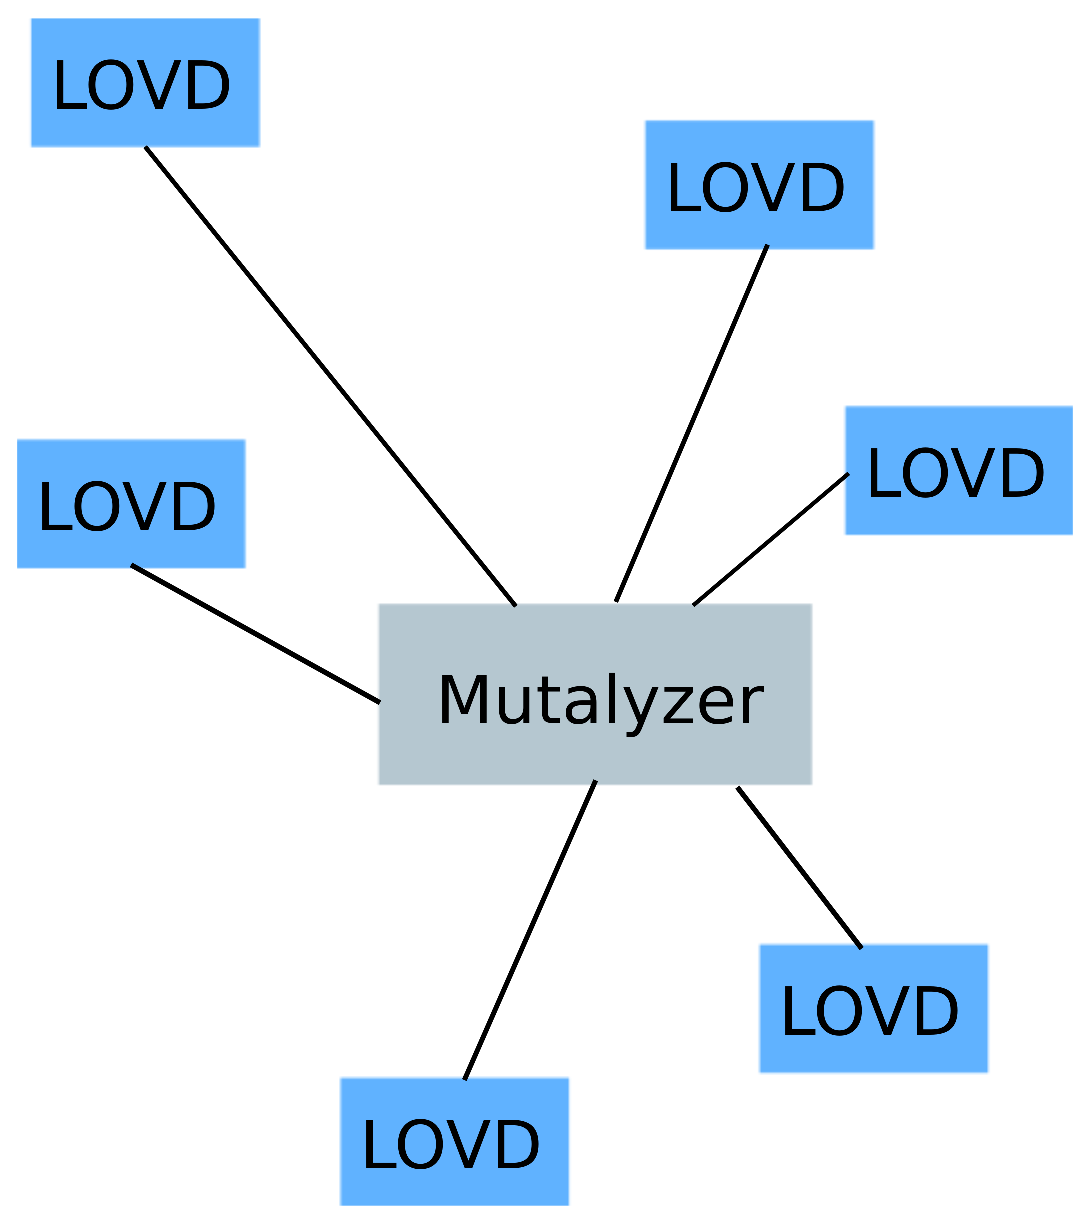
\includegraphics[scale = 0.25]{mapper}
\end{center}

The server running Mutalyzer will run the web service.

The clients will be LOVD servers.
\vfill
\end{slide}


\begin{slide}
\slideheading{Mutalyzer 1.0.4}
Mutalyzer is an LSDB curational tool.
\begin{itemize}
\item Variant nomenclature checker applying Human Genome Variation Society guidelines.
\end{itemize}

\vspace*{1cm}
Current server running:
\begin{itemize}
\item Version 1.0.4.
\item Recent stable Linux and Python versions.
\item Subversion.
\item Trac bug tracking system.
\end{itemize}
\vfill
\end{slide}

\begin{slide}
\slideheading{Mutalyzer $2.0\alpha$}
We are currently working on a new version.

\vspace*{1cm}
Complete rewrite of the code:
\begin{itemize}
\item Improved performance.
\item Restructured web interface.
\end{itemize}

Features:
\begin{itemize}
\item Context-free HGVS nomenclature parser.
\item GenBank record parser (Biopython).
\end{itemize}
\vfill
\end{slide}

\begin{slide}
\slideheading{Mutalyzer 2.0}
Planned features:
\begin{itemize}
\item Mutalyzer database check.
      \begin{itemize}
      \item Enable automatic retrieval and submission to LSDBs.
      \end{itemize}

\vspace*{1cm}
\item Implementation of:
      \begin{itemize}
      \item Extended HGVS nomenclature guidelines.
      \item LRG parsing.
      \item Automatic variant descriptions.
      \item Sequence Ontology descriptions.
      \end{itemize}
\end{itemize}
\vfill
\end{slide}

\begin{slide}
\slideheading{Mutalyzer}
Technical details of the server.

\vspace*{1cm}
\begin{itemize}
\item Lots of dependencies, most of them not present on normal web servers.
      \begin{itemize}
      \item Part of the UCSC genome browser database.
      \item Python / biopython / pyparsing.
      \item \ldots
      \end{itemize}
\item Due to modular design, capable of many tasks.
\item Capable of many requests.
\item One installation available.
\end{itemize}
\vfill
\end{slide}

\begin{slide}
\slideheading{LOVD}
Technical details of the client.

\vspace*{1cm}
\begin{itemize}
\item Designed to work on most common web servers.
\item Depends on MySQL and PHP.
\item Designed for genes (coordinates are coding sequence oriented).
\item Many independent installations $(\pm 80)$.
\end{itemize}

Chromosome oriented coordinates are needed for:
\begin{itemize}
\item Querying purposes (e.g. search all LOVD's).
\item Visualisation of mutations (e.g. all deletions in the UCSC genome 
      browser).
\end{itemize}
\vfill
\end{slide}

\begin{slide}
\slideheading{Coordinate conversion}
LOVD needs a coordinate conversion system:

\vspace*{1cm}
\begin{itemize}
\item For mapping on a chromosome, we need to convert the coding sequence
      orientated coordinates to chromosome coordinates.
\item Mutalyzer is capable of doing this.
\item Installing Mutalyzer locally is not an option.
\end{itemize}

\vspace*{1cm}
$\Rightarrow$ Make a web service.
\vfill
\end{slide}

\begin{slide}
\slideheading{Coordinate conversion}
The steps involved in this mapping are:

\vspace*{1cm}
\begin{itemize}
\item LOVD receives a new entry from a curator or submitter.
\item LOVD sends the necessary data to Mutalyzer: 
      \begin{itemize}
      \item Accession number of the used transcript (NM number).
      \item The variant (in HGVS notation).
      \end{itemize}
\item Mutalyzer processes the variant, extracts the positions.
\item Mutalyzer returns the data needed by LOVD:
      \begin{itemize}
      \item Corrected gene-orientated coordinates.
      \item Genomic coordinates.
      \item The variant type.
      \end{itemize}
\end{itemize}
\vfill
\end{slide}

\begin{slide}
\slideheading{Coordinate conversion}
Results:

\vspace*{1cm}
With these newly computed (and stored) columns, a number of new things can
be done by LOVD:

\begin{itemize}
\item Make custom tracks for use in genome browsers.
\item A more robust search for all deletions / SNPs / insertions, \ldots
\item Search for mutations within a certain range.
\item Make a web service for LOVD itself (e.g. search all LOVD's for genes
      in a range).
\item \ldots
\end{itemize}
\vfill
\end{slide}

\begin{slide}
\slideheading{Web services in LOVD (under development)}
LOVD acts as a web service itself.

\vspace*{1cm}
\begin{itemize}
\item Listing of all genes in the database.
\item Searching on the gene symbol (full match only).
\item Showing only one specific gene entry.
\item Listing of all variant entries in a certain gene.
\item Searching on the DNA position (full match only).
\item Searching on the DNA field.
\item Searching on the DBID field.
\item Showing only one specific variant entry (internal ID only).
\end{itemize}
\vfill
\end{slide}

\begin{slide}
\slideheading{Questions?}
\begin{center}
Acknowledgements

\vspace*{1cm}
Peter Taschner\\
Johan den Dunnen\\
Ivo Fokkema\\
Gerard Schaafsma\\
Jacopo Celli\\
\end{center}
\vfill
\label{LastPage}
\end{slide}

\end{document}
